%
%	Begrifflichkeiten
%

\pagebreak
\section{Nonviolent Communication}

\onehalfspacing

\subsection{Philosophical Background}

Dialectical materialism is a philosophical movement developed by Karl Marx and Friedrich Engels that explains the world in a materialistic manner, i.e., starting from material conditions.\footnote{See \textit{MIA (2022)}: Encyclopedia of Marxism. \cite{diaMat}}

It uses the dialectical method, which views contradictions and change as the driving force behind development. There are no direct "business models" in the sense of today's economic concepts that can be derived from dialectical materialism. However, certain principles of dialectical materialism can be applied to the analysis of business models to understand their contradictions and potential for development.

The dialectical method helps to analyze the development of a business model and to understand how quantitative changes (e.g., growth) can lead to qualitative leaps (e.g., new business areas).

A business model can also be negated by external influences (e.g., technological innovations) or internal developments (e.g., strategic realignment) and replaced by a new one.

\subsection{Concepts}

Concepts

\subsection{Jackal and Giraffe}

Jackal and Giraffe

\subsection{Communication Steps}

Communication Steps

\begin{figure}[H]
\centering
\caption {Four Steps}
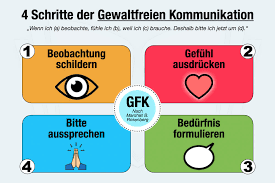
\includegraphics[width=\linewidth]{images/images.png}
\label{fig:fourSteps}
\end{figure}

\begin{figure}[H]
\centering
\caption {Examples}
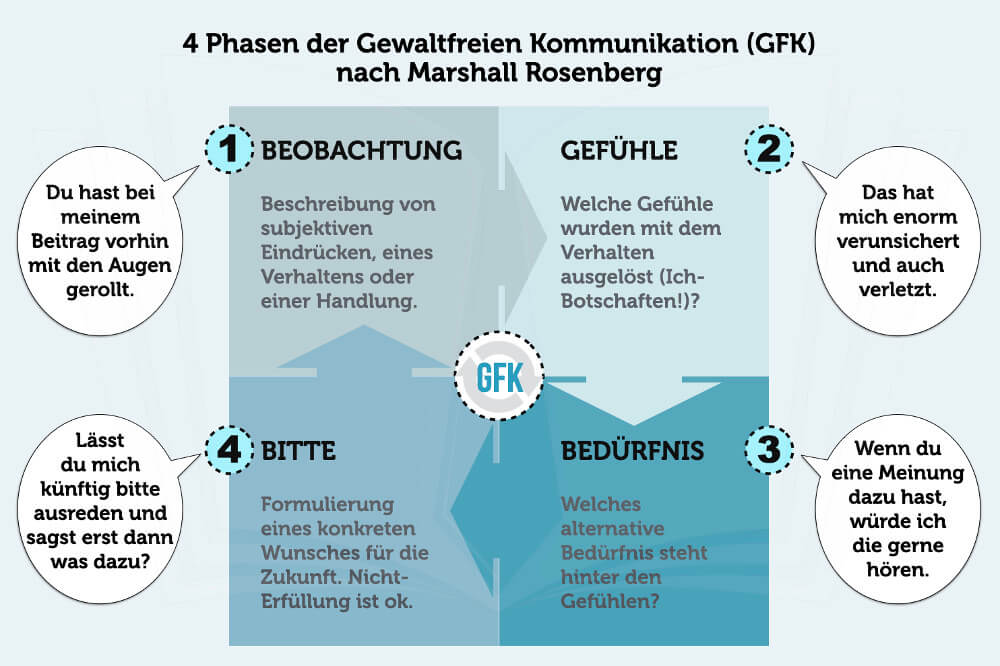
\includegraphics[width=\linewidth]{images/Gewaltfreie-Kommunikation-Beispiele.jpeg}
\label{fig:examples}
\end{figure}
